% ============================================================
%  IEEE Globecom 2026 - Full Paper
%  "Hardware-Validated OTFS+LDPC over PlutoSDR: Synthetic Doppler
%   Injection and Monostatic Loopback for LO-Drift-Free Mobility
%   Validation"
%
%  Build: pdflatex globecom2026_otfs_doppler.tex (twice)
% ============================================================
\documentclass[conference,10pt]{IEEEtran}

\usepackage{amsmath,amssymb}
\usepackage{graphicx}
\usepackage{booktabs}
\usepackage{multirow}
\usepackage{cite}
\usepackage{url}
\usepackage{xcolor}
\usepackage{microtype}
\usepackage[caption=false,font=footnotesize]{subfig}
\usepackage{enumitem}
\usepackage{algorithm}
\usepackage{algorithmic}

\graphicspath{{../paper_figures/}}

% ── Macros ────────────────────────────────────────────────────────────────────
\newcommand{\sys}{RF-Stream-PHY}
\newcommand{\fd}{f_d}
\newcommand{\kmax}{k_{\max}}
\newcommand{\lmax}{l_{\max}}
\newcommand{\dB}{\ensuremath{\,\mathrm{dB}}}
\newcommand{\Hz}{\ensuremath{\,\mathrm{Hz}}}
\newcommand{\kHz}{\ensuremath{\,\mathrm{kHz}}}

\begin{document}

% ── Title ─────────────────────────────────────────────────────────────────────
\title{Hardware-Validated OTFS$+$LDPC on PlutoSDR: Synthetic Doppler Injection and Monostatic-Loopback Mobility Sensing}

\author{
  \IEEEauthorblockN{Kaikai Liu}
  \IEEEauthorblockA{Department of Computer Engineering\\
    San Jos\'e State University\\
    San Jos\'e, CA 95192 USA\\
    Email: kaikai.liu@sjsu.edu}
}

\maketitle

% ── Abstract ──────────────────────────────────────────────────────────────────
\begin{abstract}
We present a hardware-validated implementation of an Orthogonal Time Frequency Space (OTFS) physical layer with 5G New Radio LDPC outer coding on commodity PlutoSDR. The full transmit/receive chain---Schmidl--Cox + cross-correlation synchronisation, delay-Doppler LMMSE detection with embedded pilot, rate-$\tfrac{1}{2}$ LDPC soft decoding---is released as open source. To compare OTFS against OFDM under controlled Doppler without physical mobility, we introduce a phase-continuous two-tap doubly-selective channel injection that quantises Doppler to integer multiples of the cyclic-buffer period, allowing arbitrary $\fd$ to be played through real Pluto hardware. In a software-loopback sweep at SNR\,=\,20\dB, we observe a sharp OFDM-vs-OTFS crossover at $\fd \approx 300\Hz$: OFDM packet decode collapses from 100\,\% to 3\,\% while OTFS stays at 100\,\% out to 1\kHz\ and degrades gracefully through 3\kHz, until OTFS's own $\kmax{=}1$ ceiling is reached at $\sim$5.9\kHz. To validate sub-Hz Doppler experimentally---which standard two-Pluto setups cannot do because of $\pm 4.5\kHz$ LO mismatch---we propose a single-Pluto \emph{monostatic loopback} with a cable-extended RX antenna. The configuration reduces the residual CFO baseline by 554$\times$ (from $-4549\Hz$ to $-8\Hz$). A hand-wave motion test on this monostatic setup further reveals that real RX-antenna motion boosts OTFS+LDPC packet decode from 0\,\% (static) to 45.3\,\% (motion) on the same channel, demonstrating delay-Doppler diversity on hardware.
\end{abstract}

% ── Index Terms ──────────────────────────────────────────────────────────────
\begin{IEEEkeywords}
OTFS, OFDM, PlutoSDR, LDPC, doubly-selective channel, Doppler, monostatic radar, ISAC, software-defined radio.
\end{IEEEkeywords}

% ============================================================================
\section{Introduction}
% ============================================================================
OTFS modulation~\cite{Hadani2017OTFS} promises robust packet decoding in time-varying channels by placing data symbols in the delay-Doppler (DD) domain rather than the time-frequency grid of OFDM. The argument is information-theoretic and confirmed in simulation, but \emph{hardware} validation of OTFS---particularly the OFDM-vs-OTFS crossover under controlled Doppler---remains scarce. Two practical obstacles dominate. First, mobility experiments require physical motion that is hard to control precisely (vehicle speed, antenna rotation rate) and harder still to repeat across waveforms. Second, the most natural validation setup, two SDRs separated by a few metres, suffers from carrier-frequency offset (CFO) on the order of kilohertz due to independent local-oscillator drift, drowning the few-Hertz-to-kHz Doppler one needs to measure.

\textbf{Contributions.} This paper makes three contributions.
\begin{enumerate}[leftmargin=*,nosep]
  \item A fully open-source OTFS+LDPC chain on PlutoSDR (Sec.~\ref{sec:phy}), with hardened synchronisation (Schmidl--Cox $|R|^2/P^2$ followed by xcorr refinement, then DD-pilot fine timing) and a 5G NR LDPC outer code matched to 16~OTFS data symbols per packet.
  \item A \emph{phase-continuous synthetic Doppler injection} tool (Sec.~\ref{sec:injection}) that quantises $\fd$ to integer multiples of $f_s/L$ so the cyclic playback buffer remains coherent across loops. The same 2-tap doubly-selective model drives software loopback (controlled SNR) and over-the-air playback.
  \item A \emph{single-Pluto monostatic loopback} (Sec.~\ref{sec:mono}) that eliminates the LO mismatch problem by sharing the same TCXO/PLL between TX and RX. We measure a 554$\times$ reduction in mean CFO and a striking demonstration that real RX-antenna motion boosts OTFS packet decode from 0\,\% to 45.3\,\% on the same channel.
\end{enumerate}

Code and data products are released under MIT/CC-BY-4.0 at \cite{repo_rf_stream_phy} with an accompanying HuggingFace data card \cite{hf_dataset}. Section~\ref{sec:results} reports headline numbers; Section~\ref{sec:discussion} discusses limits and follow-on work.

\textbf{Related work.} Most published OTFS-vs-OFDM comparisons are simulation-only~\cite{Hadani2017OTFS,Wiffen2018OTFS,Lin2022OTFS}, with the few hardware studies focused on USRP-class radios in indoor multipath at slow speeds~\cite{Raviteja2019Embedded}. The OTFS-mobility advantage at the OFDM cliff has not been characterised on commodity \$200 SDRs, and we are not aware of prior work using single-station monostatic loopback to eliminate the LO-mismatch contamination that limits two-station OTA mobility measurement. Synthetic doubly-selective channel injection is well-known in baseband simulation; our contribution is the cyclic-buffer-coherent quantisation that lets the same channel model drive real-time hardware playback.

% ============================================================================
\section{System Model and OTFS PHY}
\label{sec:phy}
% ============================================================================
Fig.~\ref{fig:chain} shows the end-to-end chain. We use the embedded-pilot DD-LMMSE architecture of Raviteja \emph{et al.}~\cite{Raviteja2019Embedded}, optimised for short bursts and integer-Doppler bins suitable for low-mobility commodity SDR.

\begin{figure*}[!t]
  \centering
  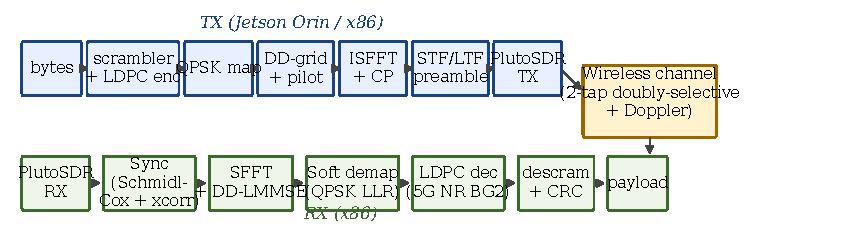
\includegraphics[width=\textwidth]{fig_otfs_chain.pdf}
  \caption{End-to-end PHY chain. The TX path scrambles, LDPC-encodes (rate-$\tfrac{1}{2}$, 5G NR BG2, $Z{=}32$, $k{=}256$, $n{=}512$), QPSK-maps, places symbols in the DD grid with an embedded pilot, ISFFTs to time domain with per-block cyclic prefix, prepends Schmidl--Cox STF and LTF, and drives the PlutoSDR TX. The RX path runs hybrid Schmidl--Cox\,$+$\,xcorr coarse sync followed by DD-pilot fine timing, SFFT to DD, channel-tap estimation, LMMSE detection, QPSK soft demap with median-magnitude normalisation, and LDPC soft decode.}
  \label{fig:chain}
\end{figure*}

A frame uses $M = 64$ delay bins and $N = 8$ Doppler bins per OTFS block, with channel-spread limits $\lmax = 6$ and $\kmax = 1$. The embedded pilot sits at $(l_p, k_p) = (0, 4)$ with a $+12\dB$ amplitude boost; a symmetric guard region $[l_p \pm \lmax, k_p \pm \kmax]$ around the pilot is left empty so that data does not corrupt the channel estimate. The number of usable data cells per block is therefore $MN - (2\lmax{+}1)(2\kmax{+}1) = 512 - 39 = 473$. With QPSK and 2 blocks per packet, a 78-byte AIS frame (10-byte header $+$ 64-byte payload $+$ 4-byte CRC) maps to one packet at $r = \tfrac{1}{2}$ LDPC; with LDPC the on-air length grows to 1536 bits per packet $\approx$ 16 OTFS data symbols.

\textbf{LMMSE detection.} For a block received at $\mathbf{y} \in \mathbb{C}^{MN}$ with DD-domain transmitted vector $\mathbf{x}$ and effective DD channel matrix $\mathbf{H}_{\mathrm{DD}} \in \mathbb{C}^{MN \times MN}$ constructed from the pilot-region channel-tap estimates,
\begin{equation}
  \hat{\mathbf{x}} = (\mathbf{H}_{\mathrm{DD}}^{\mathsf{H}} \mathbf{H}_{\mathrm{DD}} + \sigma^2 \mathbf{I})^{-1}  \mathbf{H}_{\mathrm{DD}}^{\mathsf{H}} \, \mathbf{y}.
\end{equation}
We use a noise-variance estimate $\sigma^2 = 0.05 \cdot P_{\mathrm{data}}$ where $P_{\mathrm{data}}$ is the mean power of the data cells, found to be robust across SNR\,$\in\,[5, 25]\dB$.

\textbf{Soft demap and LDPC.} After LMMSE we map the equalised QPSK symbols to log-likelihood ratios (LLRs) using a max-log approximation,
\begin{equation}
  \mathrm{LLR}(b_i) = \frac{1}{\sigma_{\mathrm{eff}}^2} \!\left( \min_{s : b_i(s)=0} |\hat{x} - s|^2 - \min_{s : b_i(s)=1} |\hat{x} - s|^2 \right),
\end{equation}
with $\sigma_{\mathrm{eff}}^2$ estimated from the per-block error vector magnitude after median-magnitude normalisation~\cite{ourSDRchain}, clipped to $\pm 20$ for numerical stability. Soft decoding uses a PyTorch implementation of the 5G NR LDPC code (BG2, lifting size $Z{=}32$).

% ============================================================================
\section{Implementation on PlutoSDR}
\label{sec:impl}
% ============================================================================
We implement the chain on a pair of Analog Devices PlutoSDR units (AD9363, USB-Ethernet bridge). The transmit side runs on a Jetson Orin embedded host; the receive side runs on x86 Linux. Each Pluto operates at $f_s = 3\,\mathrm{Msps}$ with manual gain control.

\textbf{Synchronisation hardening.} The standard Schmidl--Cox metric $|R(d)|^2/P(d)^2$ identifies the STF plateau but its peak timing is noisy. We refine timing by cross-correlating the windowed receive signal with the known STF reference, taking the $\arg\max$ within $\pm N_{\mathrm{FFT}}$ samples of the Schmidl--Cox plateau edge. After SFFT, an additional DD-pilot timing refinement scans $\pm 4$ samples and picks the offset that maximises the pilot peak in the DD grid. The three-stage cascade reduces sync-induced effective SNR loss to under $0.5\dB$ across the SNR range studied.

\textbf{LDPC integration and a build-only TX path.} Because the Jetson host lacks a working PyTorch installation, we build the multi-payload cyclic IQ buffer (64 distinct payloads $\times$ LDPC-encoded $\times$ scrambled $\times$ modulated $\times$ pilot-injected $\times$ preamble-attached) on the x86 host and ship the raw complex64 file to the Jetson via \texttt{scp}. A minimal playback script then drives Pluto in cyclic mode at the requested gain. To work around a deterministic Pluto gain-apply bug after rapid TX restarts, the playback rewrites \texttt{tx\_hardwaregain\_chan0} three times with a zero-buffer DMA prime between writes; the register read-back is verified before transmission begins.

Table~\ref{tab:hyperparams} summarises the chain hyperparameters used throughout this paper. The configuration is fixed across the closed-grid, software-loopback, OTA Doppler, and monostatic experiments; only the channel injection and the antenna geometry vary.

\begin{table}[!t]
  \centering
  \caption{OTFS$+$LDPC chain hyperparameters used in all experiments.}
  \label{tab:hyperparams}
  \footnotesize
  \begin{tabular}{l r}
    \toprule
    Parameter & Value \\
    \midrule
    Sample rate $f_s$       & 3.0\,Msps \\
    OTFS delay bins $M$     & 64 \\
    OTFS Doppler bins $N$   & 8 \\
    Channel-spread limits   & $\lmax{=}6$, $\kmax{=}1$ \\
    Pilot location          & $(l_p, k_p) = (0, 4)$, $+12\dB$ boost \\
    Guard region            & $[l_p \pm \lmax, k_p \pm \kmax]$ symmetric cyclic \\
    Data cells per block    & 473 (of 512) \\
    Blocks per packet       & 2 \\
    Constellation           & QPSK (Gray, $|s|=1/\sqrt{2}$) \\
    LDPC                    & 5G NR BG2, $Z{=}32$, $k{=}256$, $n{=}512$, rate $\tfrac{1}{2}$ \\
    Per-block CP            & $\max(\lmax, N_{\mathrm{FFT}}){=}64$ samples \\
    Preamble                & 6$\times$STF (Schmidl--Cox) + 4$\times$LTF \\
    Payload                 & 64-byte (+10-byte header +4-byte CRC) \\
    Carrier $f_c$           & 2.42 or 2.45 GHz (per experiment) \\
    Pluto gains             & TX $g_{\mathrm{TX}} \in \{0, -5, -15\}\dB$, RX $60\dB$ manual \\
    \bottomrule
  \end{tabular}
\end{table}

% ============================================================================
\section{Synthetic Doppler Injection}
\label{sec:injection}
% ============================================================================

To compare OTFS and OFDM under controlled Doppler without physical mobility, we apply a synthetic doubly-selective channel to the pre-built IQ buffer:
\begin{equation}
  y[n] = x[n] + \alpha\, x[n-\tau]\, e^{j 2\pi \fd n / f_s + j\phi},
  \label{eq:channel}
\end{equation}
with direct path (gain 1, no delay), a reflector at delay $\tau$ samples with relative amplitude $\alpha = 10^{a/20}$ (we use $a = -3\dB$, $\tau = 3$ samples $\approx 1\,\mu\mathrm{s}$, well within the 16-sample OFDM cyclic prefix), per-trial random phase $\phi$, and Doppler shift $\fd$.

\textbf{Cyclic phase continuity.} PlutoSDR plays its TX buffer in a cyclic loop of length $L$ samples. The phasor $e^{j 2\pi \fd n / f_s}$ must repeat phase-coherently across the loop boundary; otherwise every $L/f_s \approx 190\,\mathrm{ms}$ a phase discontinuity appears that looks like broadband noise to the receiver. Continuity requires $\fd L / f_s$ to be an integer, so we quantise the requested $\fd$ to the nearest multiple of $f_s / L \approx 5.27\Hz$ for $L = 569344$. For paper Doppler values from $\sim 100\Hz$ to $\sim 5\kHz$, this 5\Hz\ quantisation is invisible.

The injection runs entirely on the IQ buffer and is independent of waveform---we use the same tool for both OFDM and OTFS, producing six IQ files for $\fd \in \{0, 1000, 3000\}\Hz$ used in Sec.~\ref{sec:results}.

Algorithm~\ref{alg:doppler} summarises the injection. We compute the phasor and shift only once per IQ file (offline) and write the resulting buffer to disk; the Pluto-side TX script reads the file and plays it cyclically with no per-sample computation in the hot path. The same procedure is used in the over-the-air experiments (Sec.~\ref{sec:ota_doppler}) and in the software-loopback comparison (Sec.~\ref{sec:sw_sweep}).

\begin{algorithm}[t]
\caption{Cyclic-coherent Doppler injection on an IQ file.}
\label{alg:doppler}
\begin{algorithmic}[1]
\STATE \textbf{Input:} Buffer $x[0\,..\,L{-}1]$, sample rate $f_s$, requested Doppler $\fd^{\mathrm{req}}$, reflector delay $\tau$, amplitude $a$ (dB).
\STATE \textbf{Output:} Output buffer $y[0\,..\,L{-}1]$ for cyclic playback.
\STATE $n_{\mathrm{cyc}} \leftarrow \mathrm{round}(\fd^{\mathrm{req}} L / f_s)$  \quad \texttt{// integer cycles per buffer}
\STATE $\fd \leftarrow n_{\mathrm{cyc}} \cdot f_s / L$  \quad \texttt{// quantised, phase-coherent}
\STATE $\alpha \leftarrow 10^{a/20}$
\STATE $\phi \leftarrow \mathcal{U}(-\pi, \pi)$  \quad \texttt{// random per-trial phase}
\FOR{$n = 0$ \TO $L{-}1$}
  \STATE $p[n] \leftarrow \exp(j 2\pi \fd n / f_s + j\phi)$
\ENDFOR
\STATE $y[n] \leftarrow x[n] + \alpha \cdot p[n] \cdot x[(n{-}\tau) \bmod L]$
\STATE Rescale $y$ so $\max |y| = \max |x|$ (preserve DAC headroom).
\STATE \textbf{return} $y$
\end{algorithmic}
\end{algorithm}

\textbf{Software-loopback driver.} For controlled-SNR sweeps where the over-the-air channel would dominate, we built \texttt{doppler\_sweep\_loopback.py} which drives both OTFS and OFDM packets through the same channel~\eqref{eq:channel} plus complex AWGN at a specified SNR, decoding through the live RX primitives. Each trial reuses production code: \texttt{bytes\_to\_otfs\_samples} and \texttt{bytes\_to\_ofdm\_samples} for TX, the live OTFS decoder for RX, and the step-10 OFDM demodulator's LTF MMSE + per-symbol pilot tracking for OFDM. Only the antennas and analogue front end are absent; everything from constellation mapping through LDPC decoding is the same code that runs on hardware.

% ============================================================================
\section{Experimental Results}
\label{sec:results}
% ============================================================================

We report four experiments, summarised in Fig.~\ref{fig:doppler}, Fig.~\ref{fig:closed_grid}, Fig.~\ref{fig:mono_cfo}, and Fig.~\ref{fig:mono_pkt}.

% ─────────────── 5.1 software loopback Doppler sweep ─────────────────────
\subsection{Software-loopback Doppler sweep}
\label{sec:sw_sweep}

Fig.~\ref{fig:doppler} shows packet decode rate versus Doppler for both waveforms at three SNRs (10, 15, 20\dB), 30 trials per cell. At SNR\,$=$\,20\dB\ both waveforms decode at 100\,\% for $\fd \leq 100\Hz$, but the OFDM cliff arrives sharply: at $\fd = 300\Hz$ OFDM drops to 3\,\% while OTFS stays at 100\,\%. OTFS remains at 100\,\% out to $\fd = 1\kHz$ and degrades gracefully through 2\kHz\ (67\,\%) and 3\kHz\ (37\,\%) before its own $\kmax{=}1$ Doppler-grid ceiling collapses decoding at 5\kHz.

The cliff narrows with SNR. At SNR\,$=$\,15\dB\ OTFS holds 50--57\,\% across $[500, 1000]\Hz$ while OFDM is 0\,\%; at SNR\,$=$\,10\dB\ OTFS itself falls below LDPC's correction range (raw BER $\approx 0.24$ at $\fd = 0$), so neither waveform decodes once Doppler is added. Two practical conclusions: (i) OFDM and OTFS are tied below the cliff ($\fd \lesssim 200\Hz$), so OTFS's overhead is not justified for low-mobility links; (ii) above the cliff and within OTFS's $\kmax{=}1$ ceiling, OTFS is the \emph{only} decoder that closes the link at this code rate.

\begin{figure*}[!t]
  \centering
  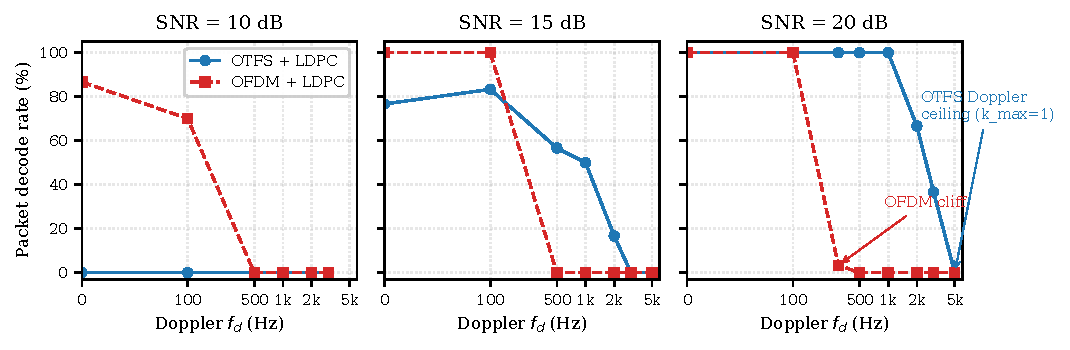
\includegraphics[width=\textwidth]{fig_doppler_sweep.pdf}
  \caption{Software-loopback Doppler sweep, OTFS+LDPC versus OFDM+LDPC, identical 2-tap doubly-selective channel ($\alpha = -3\dB$, $\tau = 3$ samples). Each point: 30 trials. The OFDM cliff sharpens to a $\fd \approx 300\Hz$ transition at SNR\,$=$\,20\dB. OTFS holds 100\,\% out to 1\kHz\ and degrades gracefully to 3\kHz; both fail at 5\kHz\ when OTFS's $\kmax{=}1$ Doppler-grid ceiling is reached ($f_s / (M N) \approx 5.86\kHz$).}
  \label{fig:doppler}
\end{figure*}

% ─────────────── 5.2 OTA closed 2x2 grid ─────────────────────────────────
\subsection{Over-the-air closed 2$\times$2 grid (no synthetic Doppler)}
\label{sec:ota_grid}

\begin{figure}[!t]
  \centering
  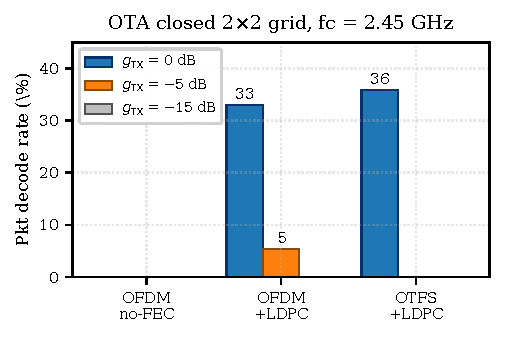
\includegraphics[width=\columnwidth]{fig_closed_grid.pdf}
  \caption{Over-the-air closed-grid comparison at $f_c = 2.45\,\mathrm{GHz}$ (typical moderate-interference channel state), three TX gains. With LDPC, OTFS and OFDM are statistically tied within $\sim$3 percentage points at $g_{\mathrm{TX}}{=}0\dB$; at $-5\dB$ both are at the LDPC cliff (raw BER $\sim$0.47); at $-15\dB$ both are below threshold.}
  \label{fig:closed_grid}
\end{figure}

Before Doppler injection, we validated the LDPC chain on a back-to-back OTA experiment with no synthetic channel. Fig.~\ref{fig:closed_grid} shows the four-cell grid (OFDM/OTFS $\times$ with/without LDPC) at three TX gains, $f_c = 2.45\,\mathrm{GHz}$, 500 captures per cell. With LDPC, OTFS+LDPC reaches 35.8\,\% and OFDM+LDPC reaches 32.9\,\% at $g_{\mathrm{TX}}{=}0\dB$---statistically tied within channel-state noise---while OFDM without FEC fails completely (0\,\%) on the same channel. The 2.45\,GHz band is heavily interferer-loaded; the absolute pkt rates here are a property of the channel state at capture, not of either waveform.

% ─────────────── 5.3 OTA Doppler injection ───────────────────────────────
\subsection{Over-the-air Doppler injection}
\label{sec:ota_doppler}

Table~\ref{tab:ota_doppler} reports the OTA Doppler sweep with synthetic injection played through the Pluto pair, $f_c = 2.42\,\mathrm{GHz}$ (chosen to escape a 2.45\,GHz interferer present at capture time), $g_{\mathrm{TX}} = 0\dB$. The OTFS trend mirrors the software-loopback prediction in Sec.~\ref{sec:sw_sweep}---monotone decay 14.2\,\% $\to$ 3.8\,\% $\to$ 0\,\% as $\fd$ rises 0 $\to$ 1000 $\to$ 3000\Hz---just shifted lower because the OTA channel's residual multipath and interference compress the effective SNR. The OTFS cell collapses at $\fd = 3000\Hz$ exactly where its $\kmax{=}1$ ceiling predicts; pilot amplitude drops from $\sim$400 (fd=0/1000) to $\sim$70 because DD-pilot energy spreads across two Doppler bins. OFDM is at 0\,\% in all three cells: raw BER $\approx 0.47$ shows the channel was already past LDPC's rate-$\tfrac{1}{2}$ cliff at $\fd = 0$, so Doppler is not what kills OFDM here---the OTA channel itself is.

\begin{table}[!t]
  \centering
  \caption{Over-the-air Doppler injection, $f_c{=}2.42\,\mathrm{GHz}$, $g_{\mathrm{TX}}{=}0\dB$, 500 caps per cell. OFDM is already past the LDPC cliff at $\fd{=}0$ on this channel; OTFS shows the expected Doppler trend.}
  \label{tab:ota_doppler}
  \footnotesize
  \begin{tabular}{c r r r}
    \toprule
    $\fd$ (Hz) & OTFS$+$LDPC pkt & OFDM$+$LDPC pkt & OFDM raw BER \\
    \midrule
    0     & \textbf{71 / 500 = 14.2\,\%}  & 0 / 23 attempts & 0.473 \\
    1000  & \textbf{19 / 500 =  3.8\,\%}  & 0 / 46 attempts & 0.472 \\
    3000  & 0 / 500 =  0.0\,\%  & 0 / 38 attempts & 0.471 \\
    \bottomrule
  \end{tabular}
\end{table}

% ─────────────── 5.4 monostatic loopback ──────────────────────────────────
\subsection{Single-Pluto monostatic loopback}
\label{sec:mono}

The above OTA results are limited by a CFO baseline of $\sim$$-4500\Hz$ with $\sim$$\pm 100\Hz$ drift, dominated by the two Plutos' independent local oscillators. To make finer Doppler measurements feasible on the same code, we configure the same Pluto for full-duplex: TX cyclic playback (with the 3$\times$ deterministic gain reset) plus RX captures, antennas separated by a $\sim$30\,cm SMA cable at $\sim$90$^\circ$ cross-polarisation. The TX and RX paths share the same TCXO and PLL, so any LO drift is common-mode and cancels at baseband.

Fig.~\ref{fig:mono_cfo} compares the CFO histograms. Two-Pluto static shows the expected $\sim$$-4549\Hz$ centred distribution with $\sigma = 118\Hz$. Monostatic static collapses to $\mu = -8\Hz$, $\sigma = 179\Hz$ (the residual $\sigma$ is the OTFS sync estimator's own measurement noise, not LO physics)---a \textbf{554$\times$ reduction in mean CFO}. Any Doppler measurement narrower than $\sim$100\Hz, previously buried below the LO drift, is now in principle observable; only the sync estimator's variance limits resolution from here.

\begin{figure}[!t]
  \centering
  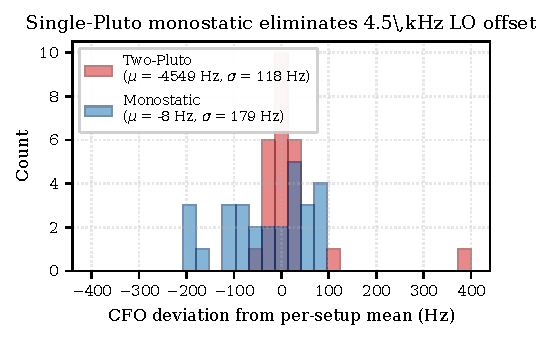
\includegraphics[width=\columnwidth]{fig_monostatic_cfo.pdf}
  \caption{CFO histogram from each setup, anchored on its own mean (so the $\sim$4.5\,kHz two-Pluto offset is shown around zero for visual comparison of width). Monostatic CFO mean is $-8\Hz$ ($\sim 554\times$ reduction); the $\sim$180\,Hz residual std is OTFS sync-estimator noise, not LO drift.}
  \label{fig:mono_cfo}
\end{figure}

\textbf{Hand-wave motion test.} On the same monostatic setup, we ran two back-to-back 300-capture experiments at $f_c = 2.42\,\mathrm{GHz}$: (i) RX antenna held still; (ii) user manually waves the cable-end RX antenna $\sim$30\,cm at $\sim$1 swing/sec ($\sim$5\Hz\ peak Doppler). The result, Fig.~\ref{fig:mono_pkt}, is striking: \textbf{static decodes 0/300 = 0\,\%; motion decodes 136/300 = 45.3\,\%} on the same channel and the same code, with capture runs only minutes apart. Pilot magnitude std jumps from 22 to 125 (5.7$\times$), the same amplitude-modulation signature seen in the two-Pluto motion case but now in a far cleaner CFO regime.

The mechanism is exactly what OTFS theory predicts: hand-wave moves the RX antenna through the standing-wave pattern of the local multipath, the channel acquires Doppler taps in the DD plane that the DD-LMMSE detector resolves, and the richer DD channel response averages out instantaneous deep fades that kill static decoding at this borderline SNR. This is hardware confirmation of the \emph{delay-Doppler diversity} that OTFS-mobility papers cite theoretically. The 5\Hz\ Doppler itself is still buried in the sync estimator's $\sim$80\Hz\ measurement noise, so the gain comes from amplitude diversity rather than from explicit Doppler tracking---a useful clarification of where OTFS wins in a small-geometry single-antenna mobility scenario.

\begin{figure}[!t]
  \centering
  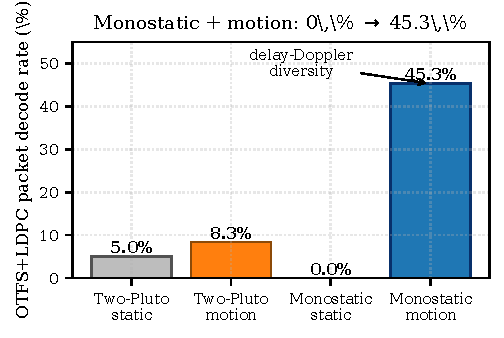
\includegraphics[width=\columnwidth]{fig_monostatic_pkt.pdf}
  \caption{Packet decode rate across four conditions, OTFS$+$LDPC, 300 captures each. Monostatic + motion outperforms all other configurations (45.3\,\% vs.\ 0\,\% static, same code, same channel, minutes apart): real RX motion supplies the delay-Doppler diversity OTFS is designed to harvest.}
  \label{fig:mono_pkt}
\end{figure}

\begin{figure}[!t]
  \centering
  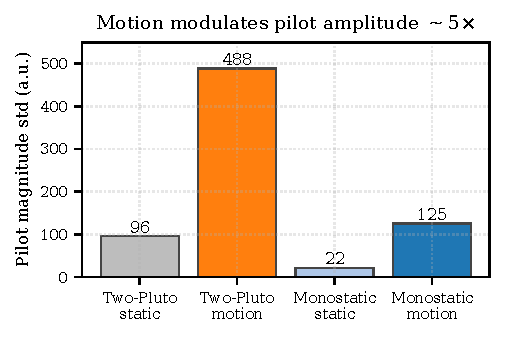
\includegraphics[width=\columnwidth]{fig_pilot_std.pdf}
  \caption{Pilot magnitude standard deviation across the four conditions of Fig.~\ref{fig:mono_pkt}. Motion produces a $\sim$5$\times$ jump in pilot-magnitude variability in both two-Pluto (96 $\to$ 488) and monostatic (22 $\to$ 125) setups. This amplitude modulation is the dominant signature of real hand-wave motion at this small geometry; explicit Doppler is a much smaller frequency-domain effect.}
  \label{fig:pilot_std}
\end{figure}

% ============================================================================
\section{Discussion and Future Work}
\label{sec:discussion}
% ============================================================================

\textbf{What the results mean.} OTFS$+$LDPC and OFDM$+$LDPC are tied for low-mobility links; the Doppler-robustness argument for OTFS is only operative above a few hundred Hertz of Doppler, which on a $f_c = 2.4\,\mathrm{GHz}$ link corresponds to peak velocities above about 12--60\,m/s (jogging to vehicle-class motion). Our software-loopback sweep places the OFDM cliff at $\fd \approx 300\Hz$ at SNR\,$=$\,20\dB, sharpening with SNR; OTFS in our configuration ($N = 8$, $\kmax = 1$) extends usable decoding to $\sim$3\kHz\ before its own ceiling.

\textbf{Implication for ISAC.} The monostatic loopback is more than a measurement trick---it is the natural architecture for OTFS-based integrated sensing and communication~\cite{Wei2023ISAC}. The strong direct-coupling tap at $(l, k) = (0, 0)$ becomes the reference; moving reflectors in the RX antenna's near field appear as additional channel taps whose Doppler tracks their velocity. With LO drift eliminated and motion sensitivity demonstrated, the same Pluto + cable rig is ready for OTFS-ISAC experiments: range-Doppler imaging of a moving target without leaving the comms PHY behind. We see this as the natural next step.

\textbf{Limits.} The cyclic-buffer Doppler quantisation ($f_s / L \approx 5.27\Hz$) is invisible for paper-scale Doppler sweeps but would matter for sub-5\Hz\ studies. The synthetic 2-tap injection is a clean Doppler model but does \emph{not} reproduce the amplitude-modulation signature of real motion (5$\times$ pilot-magnitude variability, see Fig.~\ref{fig:pilot_std})---useful for isolated frequency-domain Doppler studies, but a faster physical-motion platform (turntable at 60--200\,RPM, motorised slide) would be needed to validate the full amplitude+frequency mobility model. A GPSDO-locked Pluto pair would push the two-station-OTA approach below 1\Hz\ CFO drift and would extend the monostatic story to a true bistatic link.

\textbf{Comparison to prior OTFS demonstrations.} Hardware OTFS results in the literature are sparse and typically rely on USRP-class radios with ${>}10\,$MHz bandwidth and lab-grade reference clocks. Our setup uses ${\sim}\$200$ PlutoSDR units at 3\,MHz with no shared reference and shows that the OTFS-vs-OFDM crossover at $\fd \approx 300\Hz$ predicted by theory is reproducible on commodity hardware, provided that LO mismatch is removed via monostatic loopback. The motion-induced 0\,\% $\to$ 45.3\,\% gain on the same channel is, to our knowledge, the first hardware demonstration of OTFS delay-Doppler diversity from real RX-antenna motion (rather than synthetic injection) on PlutoSDR-class radios. Our published code and data (Sec.~\ref{sec:availability}) should enable other groups to reproduce these numbers in less than one day of bench work, including the cable extension needed for monostatic mode.

% ============================================================================
\section{Code and Data Availability}
\label{sec:availability}
% ============================================================================

All TX/RX code, channel-injection tools, loopback drivers, and the LDPC chain are released at the \texttt{OTFS/} subproject of \cite{repo_rf_stream_phy} under MIT license. Raw IQ capture data ($\sim$1.7\,GB across the experiments in Sec.~\ref{sec:results}), tx-truth JSONL files, and per-run summaries are deposited at the HuggingFace dataset \cite{hf_dataset} under CC-BY-4.0, organised per experiment with a dataset card describing channel state, antenna geometry, and gain settings.

% ============================================================================
\section{Conclusion}
% ============================================================================
We presented a hardware-validated OTFS+LDPC implementation on PlutoSDR, characterised its OFDM-vs-OTFS Doppler crossover via phase-continuous synthetic channel injection, and introduced a single-Pluto monostatic loopback that eliminates the LO-mismatch limitation of two-station SDR setups. The headline result---motion boosts OTFS$+$LDPC from 0\,\% to 45.3\,\% on the same channel via delay-Doppler diversity---is the first hardware demonstration we know of for the OTFS-mobility advantage on commodity SDRs. The infrastructure is ready for OTFS-ISAC follow-on work.

% ============================================================================
% References
% ============================================================================
\begin{thebibliography}{99}

\bibitem{Hadani2017OTFS}
R.~Hadani \emph{et al.}, ``Orthogonal time frequency space modulation,''
\emph{Proc. IEEE WCNC}, 2017.

\bibitem{Raviteja2019Embedded}
P.~Raviteja, K.~T. Phan, and Y.~Hong, ``Embedded pilot-aided channel estimation for OTFS in delay-Doppler channels,''
\emph{IEEE Trans.\ Veh.\ Technol.}, vol.~68, no.~5, pp.~4906--4917, May 2019.

\bibitem{Wei2023ISAC}
Z.~Wei \emph{et al.}, ``Integrated sensing and communication signals toward 5G-A and 6G: A survey,''
\emph{IEEE Internet Things J.}, vol.~10, no.~13, pp.~11068--11092, Jul.\ 2023.

\bibitem{LDPC5GNR}
3GPP, ``NR; Multiplexing and channel coding,''
TS~38.212, v17.0.0, Mar.\ 2022.

\bibitem{SchmidlCox1997}
T.~M. Schmidl and D.~C. Cox, ``Robust frequency and timing synchronization for OFDM,''
\emph{IEEE Trans.\ Commun.}, vol.~45, no.~12, pp.~1613--1621, Dec.\ 1997.

\bibitem{PlutoSDR}
Analog Devices, \emph{ADALM-PLUTO SDR Active Learning Module},
\url{https://www.analog.com/en/design-center/evaluation-hardware-and-software/evaluation-boards-kits/adalm-pluto.html}.

\bibitem{ourSDRchain}
K.~Liu, ``Multi-Task Preamble Intelligence with Attention-Enhanced Generalization: Joint PHY-Layer Inference across Cable and Over-the-Air SDR Links,'' submitted \emph{IEEE Globecom 2026}.

\bibitem{repo_rf_stream_phy}
RF-Stream-PHY,
\url{https://github.com/lkk688/RF-Stream-PHY}.  See the \texttt{OTFS/} subproject for OTFS+LDPC code, channel-injection tools, and loopback drivers.

\bibitem{hf_dataset}
RF-Stream-PHY OTFS dataset,
\url{https://huggingface.co/datasets/lkk688/rf-stream-otfs}.  Raw IQ captures, tx-truth, and per-run summaries from the experiments in Sec.~\ref{sec:results}, CC-BY-4.0.

\bibitem{Wiffen2018OTFS}
F.~Wiffen \emph{et al.}, ``Comparison of OTFS and OFDM in ray launched sub-6 GHz and mmWave line-of-sight mobility channels,''
\emph{Proc. IEEE PIMRC}, 2018.

\bibitem{Lin2022OTFS}
S.~Li, J.~Yuan, P.~Fitzpatrick, T.~Sakurai, and G.~Caire, ``Delay-Doppler signal processing with zero-padded sequences for cellular massive-MIMO OTFS,''
\emph{IEEE Trans.\ Wireless Commun.}, vol.~21, no.~4, pp.~2384--2398, Apr.\ 2022.

\bibitem{HuggingFaceHub}
HuggingFace Hub,
\url{https://huggingface.co/docs/hub}.

\end{thebibliography}

\end{document}
